
%%%%%%%%% MASTER -- compiles the 4 sections

\documentclass[11pt,letterpaper]{article}

\usepackage{graphicx}
\usepackage{verbatim}
\usepackage{listings}

%%%%%%%%%%%%%%%%%%%%%%%%%%%%%%%%%%%%%%%%%%%%%%%%%%%%%%%%%%%%%%%%%%%%%%%%%
\pagestyle{plain}                                                      %%
%%%%%%%%%% EXACT 1in MARGINS %%%%%%%                                   %%
\setlength{\textwidth}{6.5in}     %%                                   %%
\setlength{\oddsidemargin}{0in}   %% (It is recommended that you       %%
\setlength{\evensidemargin}{0in}  %%  not change these parameters,     %%
\setlength{\textheight}{8.5in}    %%  at the risk of having your       %%
\setlength{\topmargin}{0in}       %%  proposal dismissed on the basis  %%
\setlength{\headheight}{0in}      %%  of incorrect formatting!!!)      %%
\setlength{\headsep}{0in}         %%                                   %%
\setlength{\footskip}{.5in}       %%                                   %%
%%%%%%%%%%%%%%%%%%%%%%%%%%%%%%%%%%%%                                   %%
\newcommand{\required}[1]{\section*{\hfil #1\hfil}}                    %%
\renewcommand{\refname}{\hfil References Cited\hfil}                   %%
\bibliographystyle{plain}                                              %%
%%%%%%%%%%%%%%%%%%%%%%%%%%%%%%%%%%%%%%%%%%%%%%%%%%%%%%%%%%%%%%%%%%%%%%%%%

%PUT YOUR MACROS HERE

\date{Due February 1st, 2012}
\title{CS 395 Homework 2}

\author{Colby Blair}

\begin{document}
\maketitle

\begin{center}

Grade: \_\_\_\_\_\_\_\_\_\_\_\_\_\_\_\_\_\_\_\_
\end{center}

\thispagestyle{empty}

\pagebreak

\section*{PROBLEMS}

\subsection*{1.}
Figures \ref{merge_map} and \ref{merge_reduce} illustrate the operation of the merge sort on an array 
$ A = [3,41,52,26,38,57,9,49] $ :

\begin{figure}[!h]
        \begin{center}
                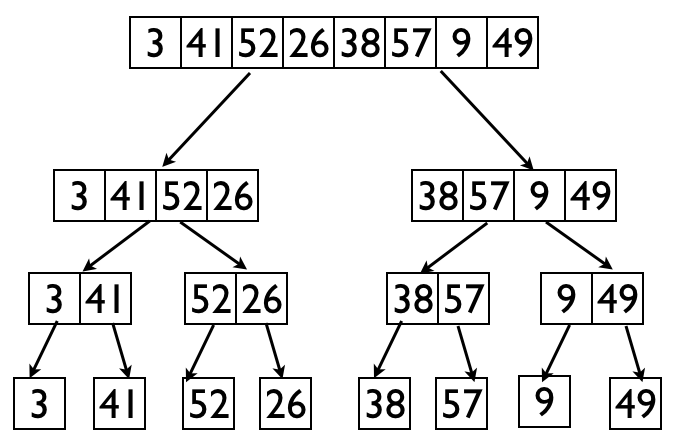
\includegraphics[width=110mm]{images/merge_map}
                \caption{Merge sort mapping down each element group}
                \label{merge_map}
        \end{center}
\end{figure}  

\begin{figure}[!h]
        \begin{center}
                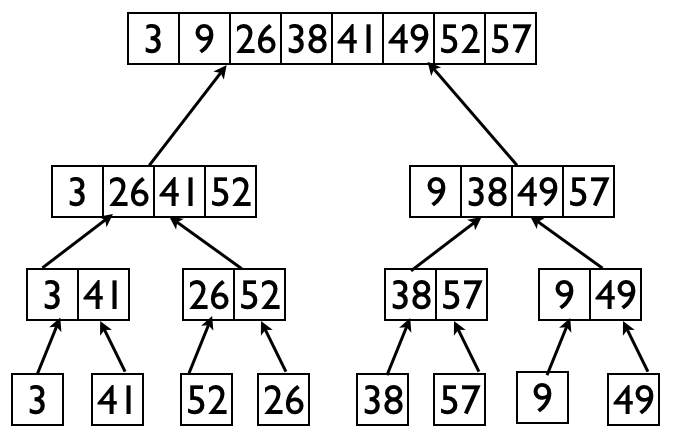
\includegraphics[width=110mm]{images/merge_reduce}
                \caption{Merge sort reducing up each element group}
                \label{merge_reduce}
        \end{center}
\end{figure} 


\subsection*{2}
\begin{figure}[!h]

\begin{lstlisting}
//merge without sentinels
merge(A, p, q, r):
	n1 = q - p + 1
	n2 = r - q
	//create arrays L and R
	L = [1 ... n1 + 1]
	R = [1 ... n2 + 1]
	for i = 1 to n1
		L[i] = A[p + i - 1]	
	for j = 1 to n2
		R[j] = A[q + j]
	i = 1
	j = 1
	for k in p to r
		//if R is empty, copy the rest of L and break
		if j == length(R)
			for i2 in i to length(L)
				A[k] = L[i2]
				i2 = i2 + 1
				k = k + 1
			return A
		//if L is empty, copy the rest of R and break
		if i == length(L)
			for j2 in j to length(L)
				A[k] = L[j2]
				j2 = j2 + 1
				k = k + 1
			return A
		if L[i] <= R[j]
			A[k] = L[i]
			i = i + 1
		else
			A[k] = R[j]
			j = j + 1
	return A
\end{lstlisting}

\caption{Merge without sentinels}
\label{merge_reduce}
\end{figure}


\pagebreak


\subsection*{3}
For an array of size $n$, there are $ n lg (n) $ levels (or recursions) in the evaluation tree, where 
$ lg (n) = log_2 (n) $ . We will show this with the following.

Assume $ n = 2^i $, with $ i $ levels having $ 2^i $ leaves. By the induction assumption, it has 
$ 2^i lg (2^i) $ levels. Notice that $ 2^i lg (2^i) = i2^i $, since $n$ has to be a power of 2. 
$ (2^i)(2^{i + 1}) = n lg (n) $ with $ n = 2^{i + 1} $. Thus, the induction step holds, demonstrating Proof by Induction. 


\subsection*{4}
The pseudocode for recursive insertion sort is as follows:

\begin{figure}[!h]

\scriptsize
\begin{lstlisting}
						C 		T
insertion_sort(A)
\end{lstlisting}

\lstset{numbers=left}
\begin{lstlisting}
	if len(A) == 1				C1		n
		return A 			C2		1
	j = length(A)				C3		n
	key = A[j]				C4		n
	A2 = A[0 ... j - 1]			C5		n
	A2 = insertion_sort(A2)			C6		n
	i = length(A2)				C7		n
	while i >= 0 and A2[i] > key:		C8		n * t1(i)
		i = i - 1			C9		(n * t1(i)) - 1
	A[i + 1] = key				C10		n
	return A2				C11		n
\end{lstlisting}
\normalsize

\caption{Recursive insertion sort}
\label{insertion_sort_rec}
\end{figure}

To find total run time $T(n)$ ($\Theta$), we total the line costs (C) and how many times they are ran (T).
In the worse case, the array $A$ is in reverse order, so $t1(i) = $, all the lengths of the subarrays being
considered:

\begin{eqnarray}
	t1(i)  	&	= \sum_{j=1}^{i} i \\
			&	= \sum_{j=1}^{n} n
\end{eqnarray}

This leads to the equation:

$ 
T(n) = nC_1 + C_2 + nC_3 + nC_4 + nC_5 + nC_6 + nC_7 + n(\sum_{j=1}^{i} i)C_8 + n((\sum_{j=1}^{i} i) - 1)C_9 + nC_{10} + nC_{11} 
$\\

$
T(n) = ( C_1 + C_3 + C_4 + C_5 + C_6 + C_7 + (\sum_{j=1}^{i} i)C_8 + ((\sum_{j=1}^{i} i) - 1)C_9 + C_{10} + C_{11})n + C_2
$\\

All the nC constants can be expressed as one constant, and we change $C_2$ to $b$:

$
T(n) = a( (\sum_{j=1}^{i} i) + (\sum_{j=1}^{i} i) - 1)n + b
$\\

$
T(n) = 2a( (\sum_{j=1}^{i} i) - 1)n + b
$\\

We can now trop the leading constants $2a$, which leaves us with $\Theta$ ( or $T(n)$) 
$ = ( ( (\sum_{j=1}^{n} n) - 1)n )$. Or simply $ = \Theta(lg(n)) $.


\pagebreak


\subsection*{5}
\begin{figure}[!h]

\scriptsize
\begin{lstlisting}
						C 		T
binary_search(A, s)
\end{lstlisting}

\lstset{numbers=left}
\begin{lstlisting}
	q = length(A) / 2			C1		1
	while length(A) > 0			C2		lg (n)
		if A[q] == s 			C3		lg (n) - 1 
			return q		C4		1
		if A[q] > s 			C5		lg (n) - 1
			A = A[1 ... q - 1]	C6		(lg (n) - 1) / 2
		else if A[q] < s 		C7		lg (n) - 1
			n = length(A)		C8		(lg (n) - 1) / 2
			A = A[q + 1 ... n]	C9		(lg (n) - 1) / 2

\end{lstlisting}
\normalsize

\caption{Iterative binary search}
\label{binary_search}
\end{figure}

Considering Figure \ref{binary_search}, we can derive the equation for total run time:

$
T(n) = C_1 + lg(n)C_2 + C_3(lg(n) - 1) + C_4 + C_5lg((n) - 1) + C_6\frac{lg(n) - 1}{2} + C_7(lg(n) - 1) + C_8\frac{lg(n) - 1}{2} + C_9\frac{lg(n) - 1}{2}
$\\

$
T(n) = C_1 + C_4 + lg(n)C_2 + ( 2C_3(lg(n) - 1) +  2C_5(lg(n) - 1) + C_6(lg(n) - 1) + 2C_7(lg(n) - 1) + C_8(lg(n) - 1) + C_9(lg(n) - 1) )
$\\

$
T(n) = C_1 + C_4 + lg(n)C_2 + ( 2C_3(lg(n) - 1) +  2C_5(lg(n) - 1) + C_6(lg(n) - 1) + 2C_7(lg(n) - 1) + C_8(lg(n) - 1) + C_9(lg(n) - 1) )
$\\

$
T(n) = C_1 + C_4 + lg(n)C_2 + (lg(n) - 1)( 2C_3 +  2C_5 + C_6 + 2C_7 + C_8 + C_9 )
$\\

$
T(n) = a lg(n) + b(lg(n) - 1) + c
$\\

We can drop the leading constant, and ignore the rest of the terms, as $ lg(n) $ is dominate as $n$ increases.
Therefore, $ \Theta(lg(n) $.
\end{document}
